\section{The AraClawBench Benchmark}
\label{sec:benchmark}

\begin{figure}[t]
    \centering
    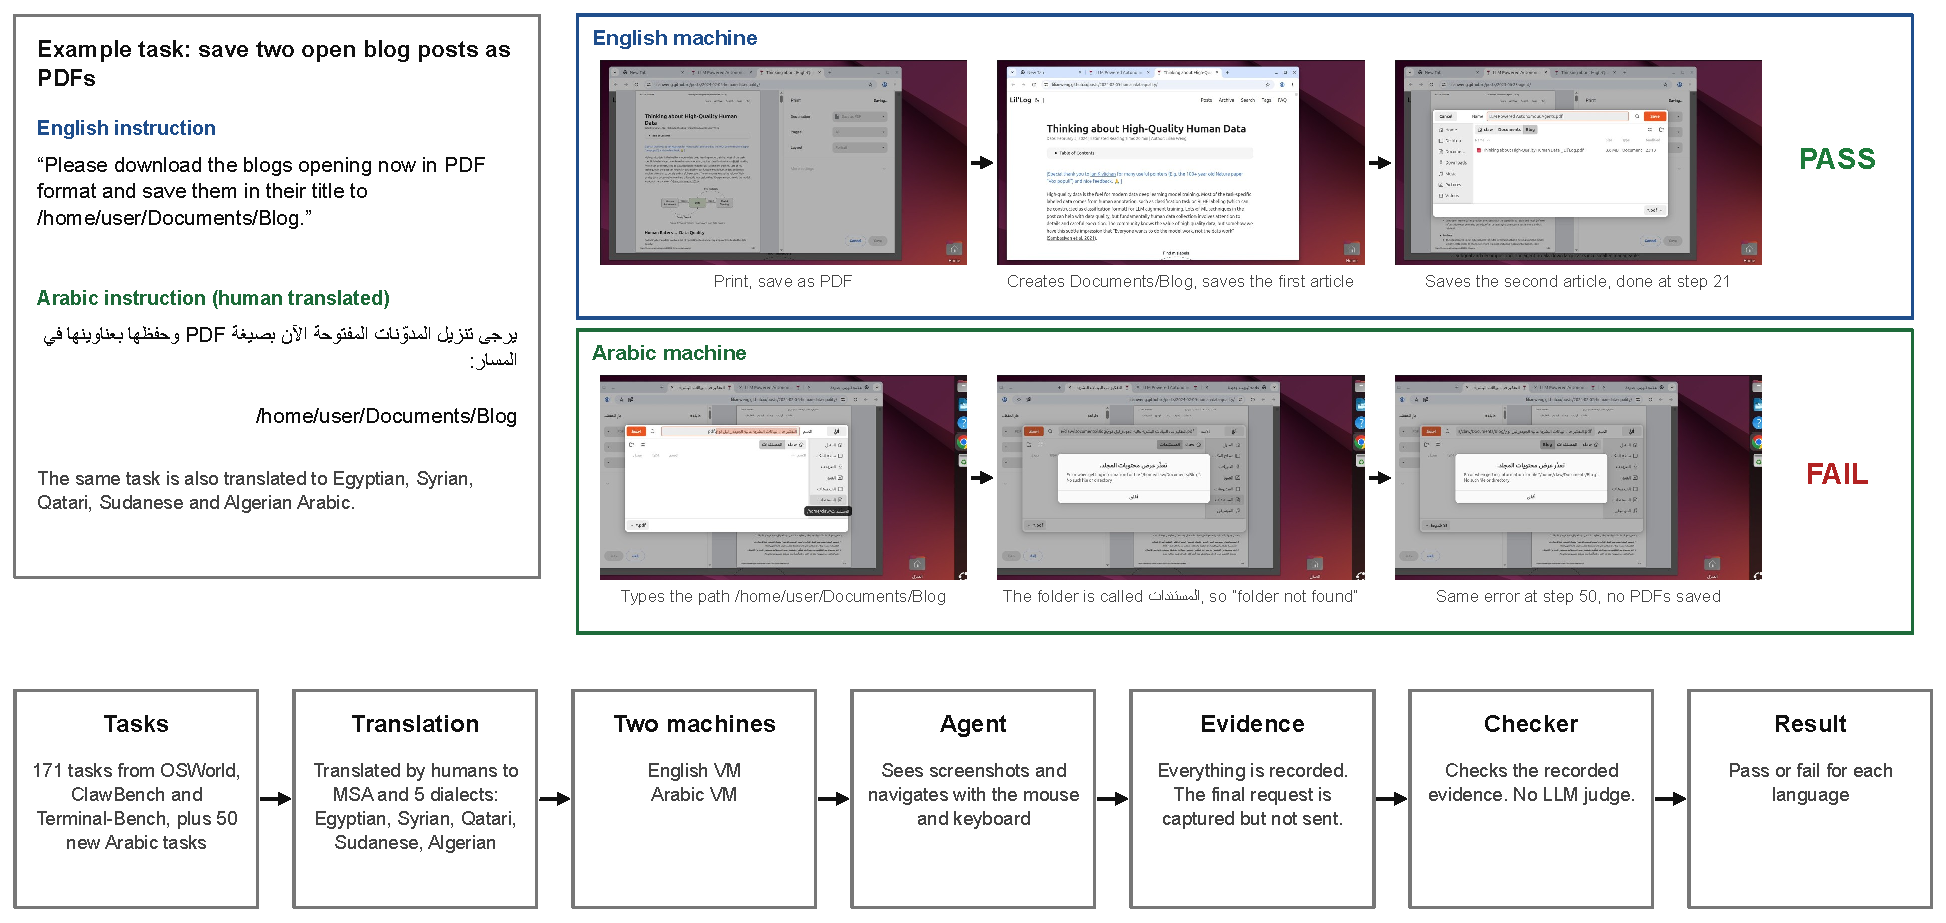
\includegraphics[width=\linewidth]{figures/fig1.pdf}
    \caption{Overview. Every task exists in English and in Arabic and runs on
    two matched virtual machines, one with an English desktop and one with an
    Arabic desktop. The agent sees only screenshots and acts through the mouse
    and keyboard. Each run is recorded and graded by a checker that reads the
    recorded evidence. The example shows a real pair: GPT-5.4 saves two blog
    posts as PDFs on the English machine, but on the Arabic machine it types the
    literal path \texttt{Documents/Blog} on a desktop whose folder is called
    \ar{المستندات} and never recovers.}
    \label{fig:overview}
\end{figure}

AraClawBench asks one question: does a computer-use agent do the same task as
well for an Arabic user as for an English user? To answer it, every task is a
pair. The English arm runs on an English computer with an English instruction.
The Arabic arm runs on an Arabic computer with the same instruction in Arabic.
Everything else is identical: the model, the step and time budget, the starting
state, and the checker. Figure~\ref{fig:overview} shows the design on one task.

\subsection{Design principles}
\label{sec:principles}

Four rules shaped every decision below. We state them once here and refer back
to them.

\textit{Same task, two languages.} The unit of measurement is a pair of runs
that differ only in language. This makes the comparison within-task, so
differences in task difficulty cancel out.

\textit{Real environments.} The Arabic arm runs on a real Arabic desktop with
Arabic folder names, an Arabic keyboard layout, right-to-left layout, and a
browser set up the way an Arab user would set it up. Web tasks run on the real
websites. We do not translate a sandbox; we measure the actual Arabic digital
environment, including its rough edges.

\textit{Evidence-based grading.} A run passes only if recorded evidence proves
it: a file with the right content, an application state, or a captured network
request. The agent's own claim of success counts for nothing. No language model
judges the primary result.

\textit{Translation fidelity.} Every Arabic instruction was translated by a
human. Anything the agent has to type or match, such as file names, quoted
titles, dates, and numbers, is kept identical in every language. This rule
exists because a mistranslated instruction produces a fake language gap
\citep{kim2026lilt}.

\subsection{Task corpus}
\label{sec:corpus}

AraClawBench has 221 tasks in three families: desktop, web, and terminal.
Table~\ref{tab:corpus} summarizes the composition.

\paragraph{Borrowed tasks.}
171 tasks come from three established benchmarks: 77 desktop tasks from
OSWorld \citep{xie2024osworld}, 76 web tasks from ClawBench
\citep{zhang2026clawbench} (39 from its first release and 37 from its second),
and 18 terminal tasks from the Terminal-Bench task pool
\citep{merrill2026terminalbench}. We selected tasks that a user in the Arab
world could plausibly want to do and that could be graded from evidence in
both languages. Six exact duplicates across sources were removed. Borrowing has
two benefits. The English arm stays comparable to published results on the
same tasks, so a reader can check our English numbers against the original
benchmarks. And the tasks arrive with their original checkers, which we reuse
wherever the evidence does not depend on language.

\paragraph{Native tasks.}
The borrowed tasks are Western tasks translated into Arabic. To also measure
the tasks an Arab user actually does, we wrote 50 new tasks: 23 web, 22
desktop, and 5 terminal. The web tasks use platforms an Arab user would use,
such as regional airlines (Qatar Airways, flydubai, Royal Jordanian), property
and shopping sites (Bayut, Ounass), a Qatari charity, Qatar Museums, an Arabic
learning platform (Edraak), and shipping and telecom services. The desktop and
terminal tasks use Arabic content: Arabic documents, Arabic spreadsheets with
Qatari invoices, Arabic-language slides, and log files from a Qatari service.
Every native task was walked end to end by hand on the real site or
application before it entered the corpus, and its grading rule was written
from what that walkthrough observed, never guessed.

\paragraph{What we could not include.}
Building the native set taught us something about the Arab web. Many regional
services (food delivery, grocery, salons, classifieds, job boards) require a
phone number verified by SMS before anything can be done, and several others
sit behind CAPTCHAs at signup. We exclude such tasks, as ClawBench does
\citep{zhang2026clawbench}, because an agent cannot legitimately pass a phone
verification. Where a whole category was walled off, we substituted a task of
similar length from a different everyday category and say so. The paper
reports the full list of excluded and substituted tasks with the reason for
each (Appendix~\ref{app:exclusions}). We treat these walls as a finding about
the ecosystem, not only as a limitation: a large share of the everyday Arab
web is closed to agents by design.

\begin{table}[t]
\centering
\small
\begin{tabular}{lrrrr}
\toprule
 & Desktop & Web & Terminal & Total \\
\midrule
Borrowed (OSWorld / ClawBench / Terminal-Bench) & 77 & 76 & 18 & 171 \\
Native (Arab-world tasks) & 22 & 23 & 5 & 50 \\
\midrule
All & 99 & 99 & 23 & 221 \\
\bottomrule
\end{tabular}
\caption{Task corpus. Every task has an English and a Modern Standard Arabic
instruction. The borrowed tasks additionally have four dialect instructions.}
\label{tab:corpus}
\end{table}

\subsection{Language arms}
\label{sec:languages}

Each task carries up to six instructions: English, Modern Standard Arabic
(MSA), and four dialects (Egyptian, Syrian, Qatari, and Sudanese). English is
the original text for borrowed tasks and the authored text for native tasks.

\paragraph{Human translation.}
The MSA instructions for all 171 borrowed tasks were produced by professional
translators and reviewed with them line by line. The dialect instructions for
the borrowed tasks were written by native speakers of each dialect. The MSA
instructions for the 50 native tasks were drafted with a language model and
reviewed by a native Arabic speaker on the team; their dialect arms were
drafted the same way and are labeled as such. We record the provenance of
every arm (human-translated, model-drafted, or model-drafted and
human-reviewed) so that results can be split by it. This matters: recent work
shows that machine-translated agent benchmarks can shift model scores by tens
of points once the translations are corrected \citep{kim2026lilt}.

\paragraph{Literal parity.}
A translation changes the language of the instruction and nothing else.
Everything the agent must type or match is pinned: file names, folder paths,
quoted strings, product names, dates, amounts, and identifiers appear verbatim
in every arm, as in the English original. Site names are kept in Latin script
with an Arabic transliteration in parentheses on first mention. A test compares
every pinned literal across all arms and fails if any differs. A second test
locks the instruction text itself: once approved, no instruction can change
without the test failing. Both tests run in continuous integration.

\paragraph{Dialects.}
Dialect arms run on the same Arabic machine as the MSA arm and are graded by
the same checker with the same Arabic answer key. The dialect changes the
voice of the instruction, never the task. This isolates the effect of
dialectal Arabic on instruction understanding from any environmental effect.

\subsection{Task packages}
\label{sec:packages}

Every task is a self-contained package with three parts.

\textit{Instructions.} The instruction strings, one per language, plus
provenance and status fields.

\textit{Setup.} What the machine looks like when the agent starts: files
placed on the desktop, applications opened, URLs loaded, and any account the
task needs. Setup is the same in both arms except for what the environment
itself localizes. A folder that is \texttt{Documents} on the English machine is
\ar{المستندات} on the Arabic one; the checker knows both.

\textit{Checker.} One success rule per task, identical in every language. The
rule is written against evidence and belongs to one of four families
(Section~\ref{sec:grading}). Where a checker needs a per-language expected
value, for example a localized folder name or a page title on a site that
serves Arabic, it carries one expected value per machine locale. Instruction
payloads never localize.

Each package also declares its budget (step and time limit), whether the task
has a consequential final action (a payment, an application, a public post)
that must be blocked, and, for tasks whose correct answer depends on live
content such as the cheapest fare on a given day, a description of the
selection condition that a secondary screenshot judge evaluates after the
deterministic check.
